% -*- latex -*-

\documentclass[twocolumn]{article}

\usepackage{amsfonts}
\usepackage{amssymb}
\usepackage{amsmath}
\usepackage{graphicx}
\usepackage{varioref}
\usepackage{fancyvrb}
\usepackage[pdfstartview=FitH]{hyperref}

\title{Divergent Color Maps for Scientific Visualization}

\author{Kenneth~Moreland}

% Commands I use for citing.
\newcommand{\lcite}[1]{~\cite{#1}}
\newcommand{\scite}[1]{~\cite{#1}}

% Avoid putting figures on their own page.
\renewcommand{\textfraction}{0.05}
\renewcommand{\topfraction}{0.95}

% Make sure this is big enough so that only big figures end up on their own
% page but small enough so that if a figure does have to be on its own
% page, it won't push everything to the bottom because it's not big enough
% to have its own page.
\renewcommand{\floatpagefraction}{.75}

\newcommand{\sticky}[1]{\textsc{[#1]}}

\begin{document}

\maketitle

\begin{abstract}
  One of the most fundamental features of scientific visualization is the
  process of mapping scalar values to colors.  This processes allows us to
  view scalar fields by coloring surfaces and volumes.  Dispite the
  importance of this mapping operation, the majority of scientific
  visualization tools and research are still using a color map that is
  famous for its ineffectiveness: the rainbow color map.  The rainbow color
  map, which na\"{i}vely sweeps through the most saturated colors a display
  can reproduce in the order of the colors in a rainbow, is well known for
  its abilities to obscure data, introduce artifacts, and confuse users.

  Although many other color maps have been proposed and used, none have
  been adopted by the visualization community as a good default in
  scientific visualization.  In this paper we explore the use of divergent
  color maps (sometimes also called bipolar color maps) for use in
  scientific visualization.  We conclude with a divergent color map that
  generally performs well in scientific visualization applications.  This
  color map is a clear replacement for the rainbow color map and can
  hopefully, once and for all, kill the use of the rainbow color map for
  serious scientific visualization applications.
\end{abstract}

\section{Introduction}
\label{sec:Introduction}

At its core, visualization is the process of providing a visual
representation of data.  One of the most fundamental and important aspects
of this process is the mapping of numbers to colors.  This mapping allows
us to pseudocolor an image or object based on varying numerical data.
Obviously, the choice of color map is important to allow the viewer to
easily perform the reverse mapping back to scalar values.

\begin{figure}
  \centering
  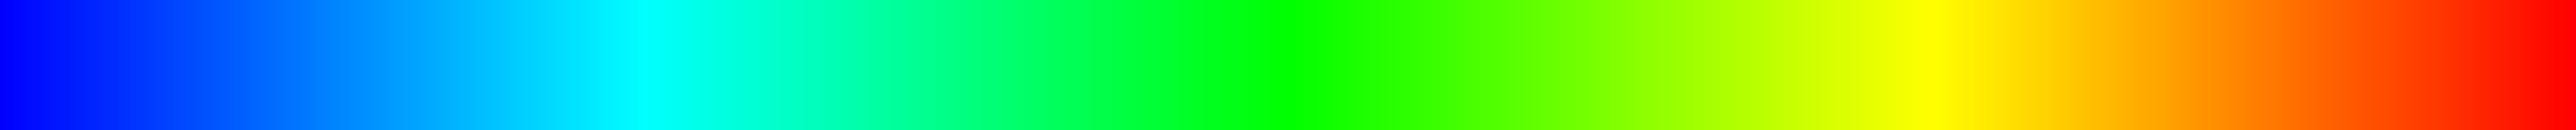
\includegraphics[width=2.5in]{images/RainbowBar}
  \caption{The rainbow color map.  Know thy enemy.}
  \label{fig:RainbowColorMap}
\end{figure}

By far the most common color map used in scientific visualization is the
rainbow color map, shown in Figure~\ref{fig:RainbowColorMap}.  In a recent
review on the use of color maps, Borland and Taylor\scite{Borland07} find
that the rainbow color map was used as the default in 8 out of the 9
toolkits they examined.  Borland and Taylor also find that in IEEE
Visualization papers from 2001 to 2005 the rainbow color map is used 51
percent of the time.

But despite its popularity, the rainbow color map has been shown to be a
poor choice for a color map in almost all problem domains.  This well
studied field of perception shows that the rainbow color map obfuscates,
rather than clarifies, the display of data in a variety of ways.  The
choice of a color map can be a complicated decision that changes based on
the visualization type and problem domain, but the rainbow color map is a
poor choice in almost all of them.

So why are so many visualization scientists and developers, experts who
should know better, still using the rainbow color map?  The answer is
unknown; there are many contributing factors.  Surely two main factors
heavily contribute.  The first is the ease at which the rainbow color map
can be created.  I myself am guilty of creating my first rainbow color map
long before learning anything about color spaces and human perception.  It
was my first choice and I was pleased with the colorful images, ignorant of
their dubious scientific value.

A second major contributor to the dominance of the rainbow color map is the
lack of a clear alternative, especially in terms of scientific
visualization.  There are certainly many publications that recommend some
very good choices for color maps\lcite{Ware04}\sticky{Site
  Brewer. Tufte?}.  However, each has its sets of features and detractors,
and the choice of the ``right'' one is difficult.

This paper is a concluding report on the quest for finding a good default
color map for a general purpose scientific visualization application.  The
color map derived here is an all-around good performer: it works well for
low and high frequency data, orders the data, is perceptually linear,
behaves well for observers with color-deficient vision, and has reasonably
low impact on the shading of three dimensional surfaces.


\section{Previous Work}
\label{sec:PreviousWork}

This previous work section is divided into two parts.  The first part is a
quick review on previously proposed color maps and lists the benifits and
detractors of each.  The second section is a quick review on color spaces,
which are used heavily in the subsequent discussions in this paper.

\subsection{Color Maps}
\label{sec:PreviousWork:ColorMaps}

\begin{figure}
  \centering
  
\includegraphics[width=2.5in]{images/GrayscaleBar}
  \caption{The grayscale color map.}
  \label{fig:GrayscaleColorMap}
\end{figure}

Let us start with perhaps the simplest color map of all: the grayscale
color map shown in Figure~\ref{fig:GrayscaleColorMap}.  Completely devoid
of any chromaticity, this map relies entirely on luminance to demonstrate
the numerical value.  Although a very simple map to create and use, this
map is surprisingly effective as the human visual system is most sensitive
to changes in luminance\sticky{Find the appropriate reference.  I think
  Ware's book might have this.  Rogowitz might also mention this.}.  The
grayscale color map is used heavily in the image processing and medical
visualization fields.

\begin{figure}
  \centering
  
\includegraphics[width=2.5in]{images/GrayscaleLocality}
  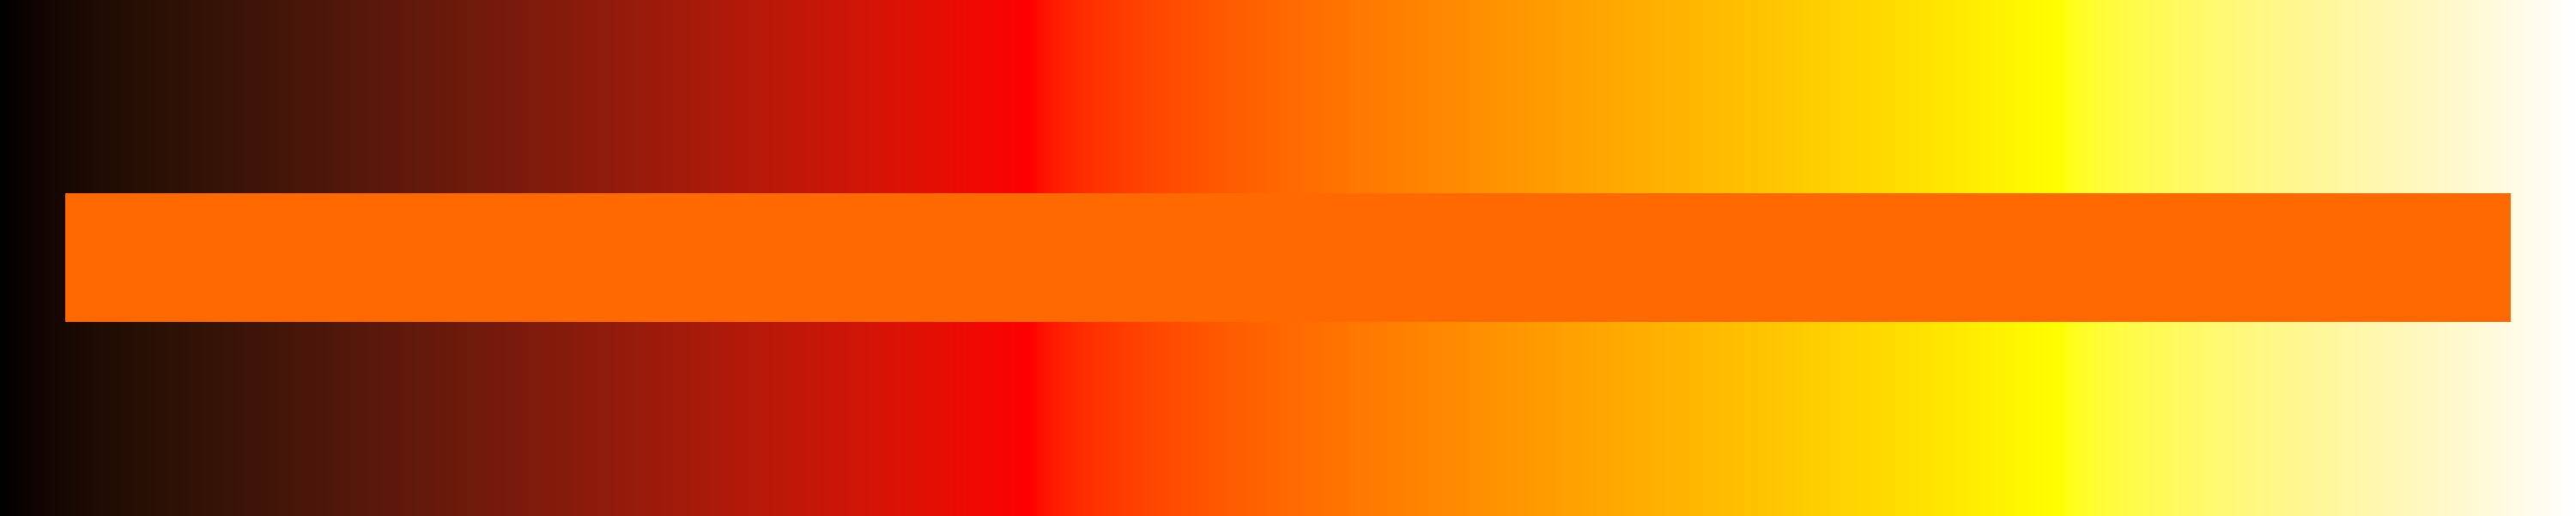
\includegraphics[width=2.5in]{images/BlackBodyLocality}
  \caption{Pixels of the same luminance may look different depending on the
    surrounding pixels (as demonstrated on the top), but color perception
    is relatively stable (as demonstrated on the bottom).}
  \label{fig:GrayscaleLocality}
\end{figure}
The grayscale color map also has a couple of detractors.  One problem is
that a human's perception to brightness is subject to the brightness of the
surrounding area.  Thus, when asked to compare the luminance of two objects
separated by distance and background, human subjects error up to 20\%.
This effect is demonstrated in Figure~\ref{fig:GrayscaleLocality}.  The
problem can be corrected by adding a chromaticity shift.

% \begin{figure}
%   \centering
%   \includegraphics[width=1.25in]{images/GrayscaleDiscontinuity}
%   \qquad
%   \includegraphics[width=1.25in]{images/RainbowDiscontinuity}
%   \caption{A discontinuity in the data is easily visible with a grayscale
%     color map (left) but is completely hidden by the rainbow color map
%     (right).  Instead, the rainbow color map appears to show variation in
%     the cyan and yellow regions that do not exist.}
%   \label{fig:discontinuity}
% \end{figure}

\subsection{Color Spaces}
\label{sec:PreviousWork:ColorSpaces}

\section{Acknowledgements}


This work was done at Sandia National Laboratories.  Sandia is a
multiprogram laboratory operated by Sandia Corporation, a Lockheed Martin
Company, for the United States Department of Energy's National Nuclear
Security Administration under contract DE-AC04-94AL85000.

\bibliographystyle{plain}
\bibliography{ColorMaps}

\end{document}
